\chapter{Manuale per l'uso \emoji{closed-book}}

In questo capitolo viene presentato il manuale per l'uso del software S.P.Q.R. (\textit{Selective Protocol for Quality and Reliability}) nel quale vengono riportati i principali esempi di funzionamento, con l'obiettivo di illustrare il comportamento del server e dei client in risposta ai comandi inviati.

\section{Introduzione}
Per facilitare la distribuzione e l'utilizzo del software, è stato redatto un manuale d'uso che descrive le funzionalità principali del progetto.
Il manuale è suddiviso in sezioni, ognuna delle quali descrive un aspetto specifico del software.
In particolare, quest'ultimo fornisce informazioni su come installare e configurare il software, con un focus particolare sulle funzionalità offerte dal server e dai client.
Inoltre vengono forniti esempi di utilizzo dei comandi principali, al fine di illustrare il comportamento del sistema in risposta alle richieste degli utenti.
Infine è possibile contribuire al progetto, segnalando eventuali bug o suggerendo nuove funzionalità da implementare, attraverso il \href{https://github.com/AntonioBerna/spqr}{repository GitHub ufficiale}.

\subsection{Download e installazione}
Per installare il software S.P.Q.R. è necessario scaricare il codice sorgente.
Per fare ciò, è possibile clonare il repository GitHub del progetto, eseguendo il seguente comando da terminale:

\begin{lstlisting}[numbers=none]
git clone https://github.com/AntonioBerna/spqr.git
\end{lstlisting}

al termine del download, è possibile accedere alla directory del progetto, eseguendo il comando:

\begin{lstlisting}[numbers=none]
cd spqr/
\end{lstlisting}

All'interno di quest'ultima è presente il file \lstinlinebg{Makefile}, che permette di compilare il codice sorgente e generare i file eseguibili.
In particolare, sono disponibili i seguenti comandi:

\begin{lstlisting}[style=bash,language=bash,numbers=none]
make        # Compilazione del codice sorgente in release mode
make debug  # Compilazione del codice sorgente in debug mode
make clean  # Pulizia dei file generati dalla compilazione
\end{lstlisting}

La compilazione in release mode è consigliata per l'utilizzo del software in produzione, mentre la compilazione in debug mode è utile per il testing e il debugging del codice, in quanto abilita la stampa di messaggi di log aggiuntivi.
Una volta che il codice sorgente è stato compilato con successo viene generata una directory \lstinlinebg{bin/}, all'interno della quale sono presenti i file eseguibili \lstinlinebg{spqr-server} e \lstinlinebg{spqr-client}.
In particolare, se tutto è andato a buon fine, si ottiene il seguente output:

\begin{lstlisting}[numbers=none]
Build in release mode completed. Run with ./bin/spqr-server and ./bin/spqr-client <IPv4>
\end{lstlisting}

\subsubsection{Installazione avanzata}
Per impostazione predefinita, il software S.P.Q.R. viene compilato utilizzando il compilatore \lstinlinebg{clang} con alcune opzioni di compilazione predefinite, che per semplicità sono riportate di seguito:

\begin{lstlisting}[numbers=none]
CC=clang
CFLAGS=-Wall -Wextra -Werror -pedantic
\end{lstlisting}

Lo stesso discorso vale per la directory di output, che viene impostata di default come segue:

\begin{lstlisting}[numbers=none]
BINARY_DIR=bin/
\end{lstlisting}

Tuttavia, è possibile personalizzare le opzioni di compilazione e la directory di output, modificando il file \lstinlinebg{Makefile} e aggiungendo le opzioni desiderate, tenendo presente che il software è stato testato con successo utilizzando il compilatore \lstinlinebg{clang} e le opzioni di compilazione predefinite.

\subsection{Disinstallazione}
Per disinstallare definitivamente il software S.P.Q.R. è sufficiente eliminare la directory del progetto, eseguendo il seguente comando da terminale:

\begin{lstlisting}[numbers=none]
rm -r spqr/
\end{lstlisting}

Invece, per pulire i file generati dalla compilazione e mantenere solo i file sorgente, è possibile eseguire il comando:

\begin{lstlisting}[numbers=none]
make clean
\end{lstlisting}

\subsection{Configurazione del software}
Il software S.P.Q.R. è stato progettato per essere configurabile, in modo da adattarsi alle esigenze degli utenti, infatti è possibile configurarlo modificando i parametri presenti nel file \lstinlinebg{include/settings.h}.
In particolare è possibile configurare la porta di ascolto del server:

\begin{lstlisting}[language=C,numbers=none,keywords={define}]
#define PORT 6969
\end{lstlisting}

scegliendo un valore compreso tra \lstinlinebg{1024} e \lstinlinebg{65535}.
Inoltre è possibile configurare il percorso delle directory del server e del client, avendo cura di modificare non solo il nome della directory, ma anche di aggiungere il carattere \lstinlinebg{/} alla fine del percorso:

\begin{lstlisting}[language=C,numbers=none,keywords={define}]
#define SERVER_FILES_PATH "server-files/"
#define CLIENT_FILES_PATH "client-files/"
\end{lstlisting}

Per impostazione predefinita, quando si scarica il codice sorgente del progetto, le directory \lstinlinebg{server-files/} e \lstinlinebg{client-files/} sono presenti nella directory principale del progetto.
Tuttavia se si decide di modificare il nome delle directory o il percorso, è necessario assicurarsi che le directory esistano e siano accessibili in lettura e scrittura.
\'E possibile configurare il simbolo che identifica i pacchetti:

\begin{lstlisting}[language=C,numbers=none,escapeinside={(*}{*)},keywords={define}]
#define PACKAGE_EMOJI "(*\emoji{package}*)"
\end{lstlisting}

il timeout statico, il timeout adattivo, la dimensione della finestra, la probabilità di perdita dei pacchetti, il numero massimo di errori prima della chiusura della connessione, il timeout di connessione e il numero di tentativi di connessione:

\begin{lstlisting}[language=C,numbers=none,keywords={define}]
#define TIMEOUT             8000  // ? Configurable Static Timeout (8 ms)
#define LOSS_PROBABILITY    25    // ? Range [0, 80]
#define WINDOW_SIZE         32    // ? Range [8, 128]
#define ADAPTIVE            true  // ? Configurable Adaptive Timeout
#define TIME_UNIT           4000  // ? 4 ms
#define MAX_TIMEOUT         80000 // ? 80 ms
#define MIN_TIMEOUT         8000  // ? 8 ms
#define MAX_ERRORS          25    // ? Maximum errors before closing the connection
#define TIMEOUT_CONNECTION  3600  // ? 1 hour
#define CONNECTION_ATTEMPTS 3     // ? Number of connection attempts
\end{lstlisting}

\subsection{Esecuzione del software e comandi disponibili}
Una volta che il software è stato compilato in release mode con successo, è possibile eseguire il server e i client, utilizzando la seguente procedura.
Innanzitutto è necessario avviare il server utilizzando il seguente comando:

\begin{lstlisting}[numbers=none]
./bin/spqr-server
\end{lstlisting}

ottenendo:

\begin{lstlisting}[numbers=none,escapeinside={(*}{*)}]
 ____           ____            ___              ____  
/ ___|         |  _ \          / _ \            |  _ \ 
\___ \         | |_) |        | | | |           | |_) |
 ___) |        |  __/         | |_| |           |  _ < 
|____/elective |_|rotocol for  \__\_\uality and |_| \_\eliability

    Developed by Antonio Bernardini & Flavio Caporilli

(*\emoji{globe-with-meridians}*) Server is listening for incoming connections.
\end{lstlisting}

Il server per impostazione predefinita utilizza l'indirizzo IPv4 \lstinlinebg{127.0.0.1} (localhost) e la porta \lstinlinebg{6968}, finchè rimane in attesa di connessioni da parte dei client.
La porta \lstinlinebg{6968} è dedicata all'attesa della connessione da parte di un client, mentre la porta \lstinlinebg{6969} viene utilizzata per il trasferimento dei file e per lo scambio di messaggi tra il server e il primo client connesso.
Di conseguenza, ogni client che si collega riceverà una porta specifica: il secondo client sarà assegnato alla porta \lstinlinebg{6970}, il terzo alla \lstinlinebg{6971} e così via.
Quando un client si connette al server con successo, il server stampa il seguente messaggio:

\begin{lstlisting}[numbers=none]
The client #0 is connected on port 6969.
\end{lstlisting}

Mentre, per avviare un client è necessario eseguire il seguente comando:

\begin{lstlisting}[numbers=none]
./bin/spqr-client <IPv4>
\end{lstlisting}

ottenendo:

\begin{lstlisting}[numbers=none,escapeinside={(*}{*)}]
 ____           ____            ___              ____  
/ ___|         |  _ \          / _ \            |  _ \ 
\___ \         | |_) |        | | | |           | |_) |
 ___) |        |  __/         | |_| |           |  _ < 
|____/elective |_|rotocol for  \__\_\uality and |_| \_\eliability

Developed by Antonio Bernardini & Flavio Caporilli

(*\emoji{globe-with-meridians}*) Connection established with the server.
\end{lstlisting}

dove \lstinlinebg{<IPv4>} è l'indirizzo IPv4 del server, ad esempio \lstinlinebg{127.0.0.1} (localhost), per connettersi al server in locale, oppure \lstinlinebg{10.2.2.15} per connettersi ad una macchina virtuale in rete.
A differenza del server, i client forniscono i parametri di configurazione utilizzati per la connessione:

\begin{lstlisting}[numbers=none]
    ╔══════════════════════════╗
    ║ CONFIGURATION PARAMETERS ║
    ╠══════════════════════════╣
    ║ WINDOW_SIZE      = 32    ║
    ║ LOSS_PROBABILITY = 25%   ║
    ║ TIMEOUT          = 8000  ║
    ║ ADAPTIVE         = true  ║
    ╚══════════════════════════╝
\end{lstlisting}

ed inoltre forniscono un prompt interattivo, che permette di inviare i comandi al server:

\begin{lstlisting}[numbers=none,escapeinside={(*}{*)}]
    ╔═══════════╦══════════════════════════════════════════╗
    ║  Command  ║                Description               ║
    ╠═══════════╬══════════════════════════════════════════╣
    ║ (*\emoji{card-index-dividers}*) LIST   ║ List the files available on the server   ║
    ╠═══════════╬══════════════════════════════════════════╣
    ║ (*\emoji{inbox-tray}*) GET    ║ Download a file from the server          ║
    ╠═══════════╬══════════════════════════════════════════╣
    ║ (*\emoji{outbox-tray}*) PUT    ║ Upload a file to the server              ║
    ╠═══════════╬══════════════════════════════════════════╣
    ║ (*\emoji{cross-mark}*) CLOSE  ║ Close the connection                     ║
    ╚═══════════╩══════════════════════════════════════════╝

    [client@spqr ~]$
\end{lstlisting}

Si noti la presenza del comando \lstinlinebg{CLOSE}, che permette di chiudere la connessione tra il server e il client.
In particolare il client viene terminato correttamente:

\begin{lstlisting}[numbers=none,escapeinside={(*}{*)}]
[client@spqr ~]$ close

Bye bye! (*\emoji{wave}*)
\end{lstlisting}

mentre il server rimane in attesa di connessioni da parte di altri client, annotando nella memoria condivisa che si è liberata una posizione, utilizzando il seguente messaggio:

\begin{lstlisting}[numbers=none]
Closed connection for client #0 on port 6969 with exit code 0.
\end{lstlisting}

Infine si noti la presenza degli altri comandi \lstinlinebg{LIST}, \lstinlinebg{GET} e \lstinlinebg{PUT}, che permettono di listare i file disponibili sul server, scaricare un file dal server e caricare un file sul server, rispettivamente.

\section{Esempi di funzionamento}

\subsection{Esempio d'uso del comando \lstinlinebig{LIST}}

Una volta che la connessione client-server è stata stabilita con successo, è possibile utilizzare il comando \lstinlinebg{LIST} per ottenere la lista dei file disponibili sul server:

\begin{lstlisting}[numbers=none,escapeinside={(*}{*)}]
[client@spqr ~]$ list

List of files availables on the server:
  (*\emoji{books}*) Progetto2324.pdf
  (*\emoji{open-file-folder}*) README.md
  (*\emoji{page-facing-up}*) GuidaC.txt
\end{lstlisting}

\subsubsection{Analisi del traffico di rete \emoji{shark}}

Solo per questo esempio, poichè è il più semplice e intuitivo, si è deciso di mostrare il risultato del comando \lstinlinebg{LIST} analizzando il traffico di rete.
Un metodo interessante per fare ciò è di utilizzare il tool \textit{Wireshark}.
In particolare, simuliamo lo scenario in cui viene instaurata la connessione client-server, viene inviato il comando \lstinlinebg{LIST}, quindi il server risponde con la lista dei file disponibili, ed infine viene chiusa la connessione.
Il \textit{Three-Way Handshake} apre la connessione tra il client e il server utilizzando la sequenza di pacchetti \lstinlinebg{SYN}, \lstinlinebg{SYN-ACK} e \lstinlinebg{ACK}, come mostrato in Fig. \ref{fig:syn-synack-ack}.

\begin{figure}[h]
    \centering
    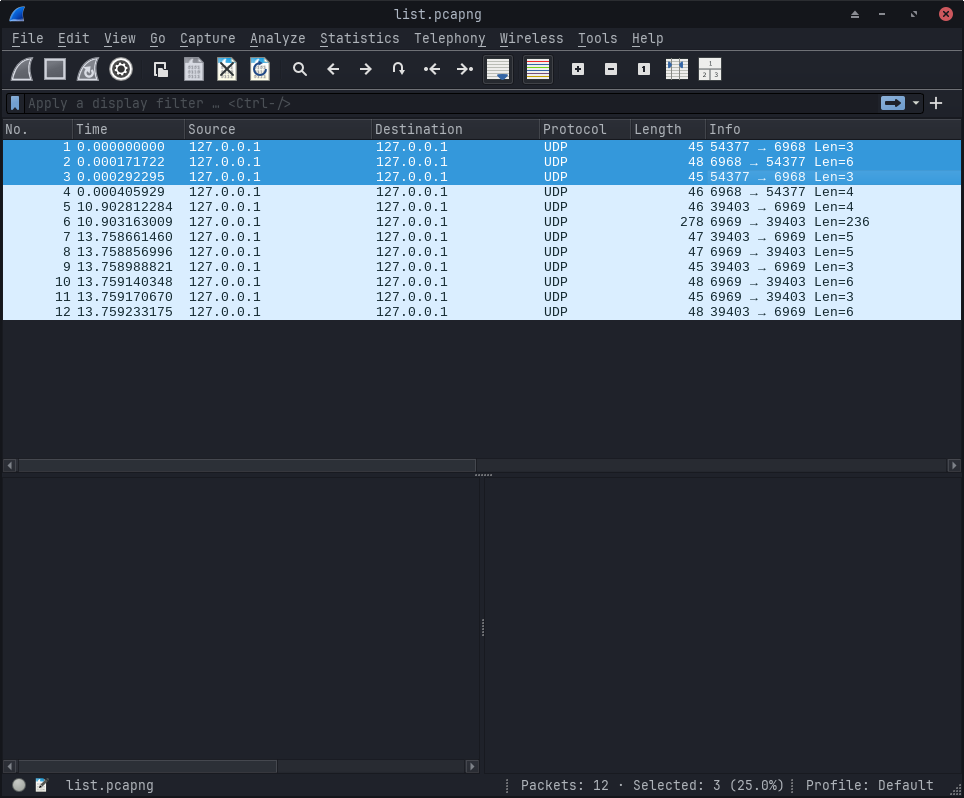
\includegraphics[width=0.6\textwidth]{imgs/03/syn-synack-ack.png}
    \caption{Three-Way Handshake: \lstinlinebg{SYN}, \lstinlinebg{SYN-ACK} e \lstinlinebg{ACK}}
    \label{fig:syn-synack-ack}
\end{figure}

successivamente, dopo che il server si è duplicato (tramite la funzione \lstinlinebg{fork()}) viene inviata la porta \lstinlinebg{6969} dal server al client, come mostrato in Fig. \ref{fig:port-6969}.

\begin{figure}[h]
    \centering
    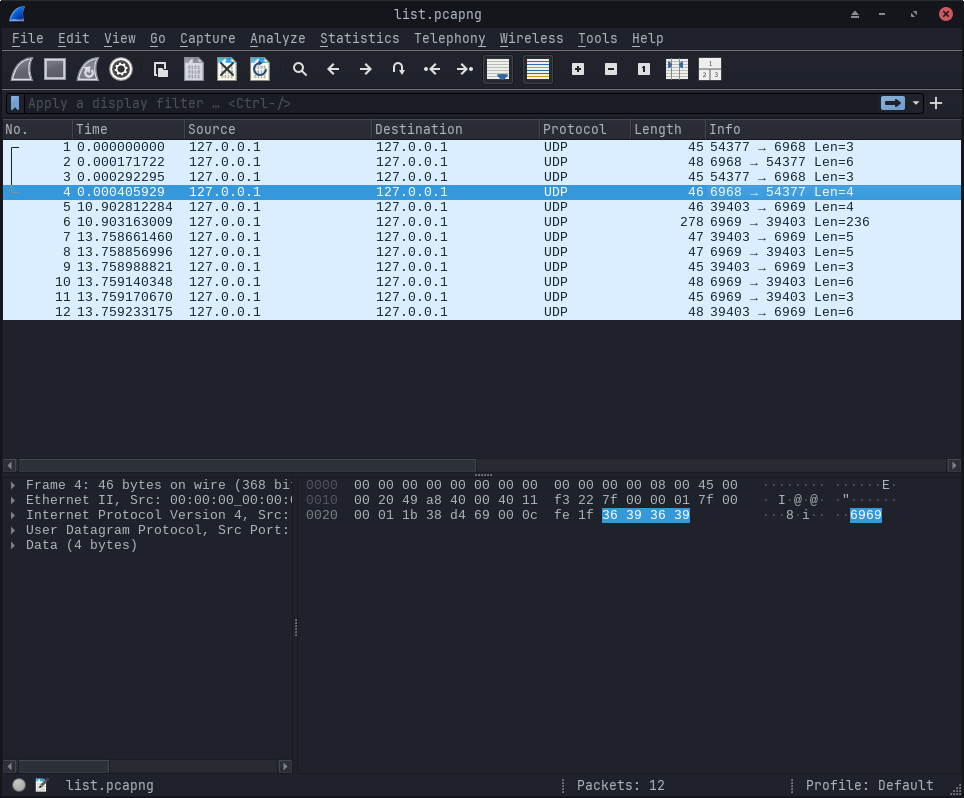
\includegraphics[width=0.6\textwidth]{imgs/03/port.png}
    \caption{Porta \lstinlinebg{6969} inviata dal server al client}
    \label{fig:port-6969}
\end{figure}

Il server risponde con la lista dei file disponibili, come mostrato in Fig. \ref{fig:list}.

\begin{figure}[h]
    \centering
    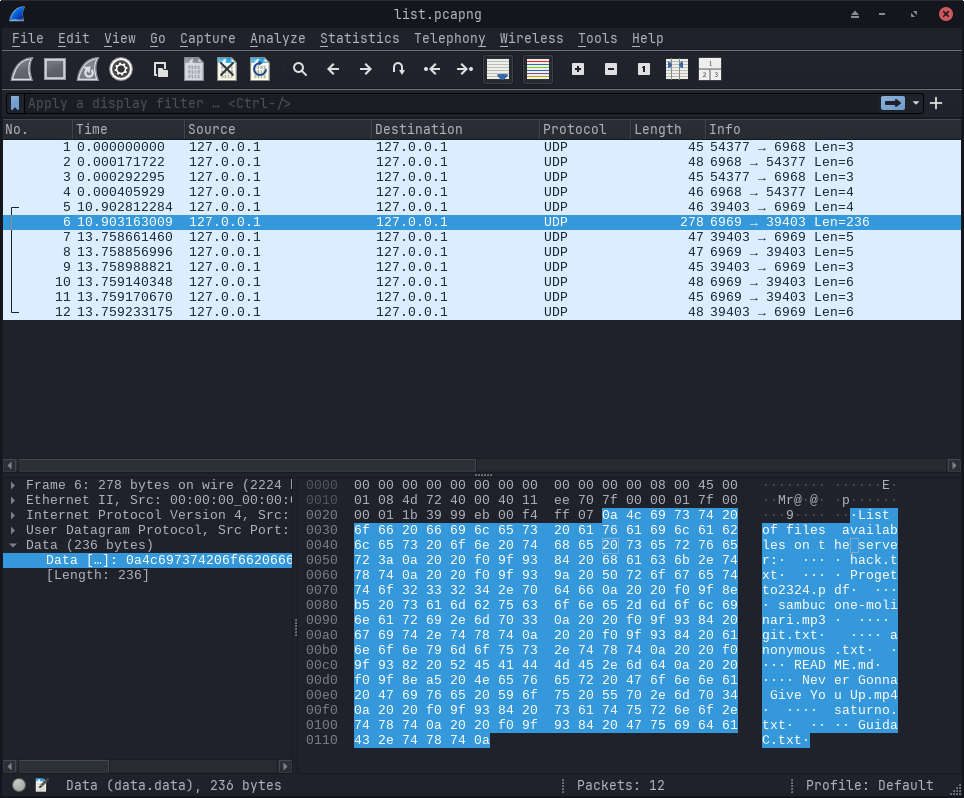
\includegraphics[width=0.6\textwidth]{imgs/03/list-cmd.png}
    \caption{Lista dei file disponibili inviata dal server al client}
    \label{fig:list}
\end{figure}

Infine viene chiusa la connessione tra il client e il server.
In particolare viene usato il comado \lstinlinebg{CLOSE} per chiudere la connessione, tramite i pacchetti \lstinlinebg{FIN}, \lstinlinebg{FIN-ACK}, \lstinlinebg{FIN} e \lstinlinebg{FIN-ACK}, come mostrato in Fig. \ref{fig:fin-finack-ack}.

\begin{figure}[h]
    \centering
    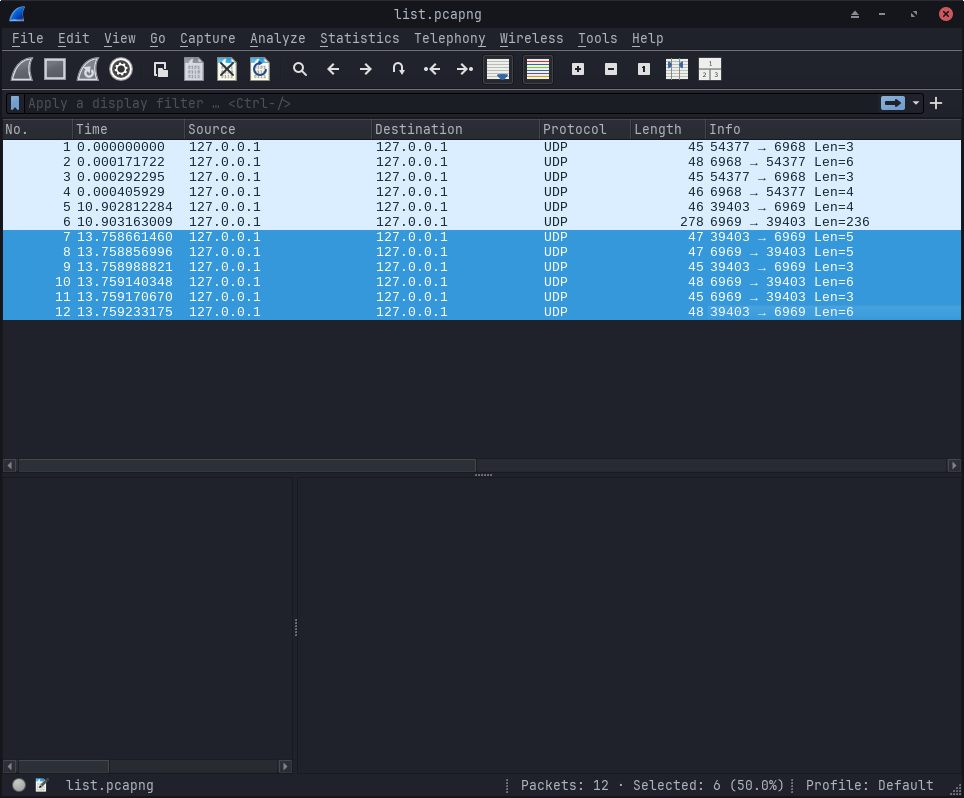
\includegraphics[width=0.6\textwidth]{imgs/03/close-CLOSE-fin-finack-fin-finack.png}
    \caption{Three-Way Handshake: \lstinlinebg{CLOSE}, \lstinlinebg{FIN}, \lstinlinebg{FIN-ACK}, \lstinlinebg{FIN} e \lstinlinebg{FIN-ACK}}
    \label{fig:fin-finack-ack}
\end{figure}

\subsection{Esempio d'uso del comando \lstinlinebig{GET}}
Utilizzando il comando \lstinlinebg{GET} è possibile effettuare il download di un file dal server.
Per usare tale comando è richiesto l'utilizzo del comando \lstinlinebg{LIST} per ottenere la lista dei file disponibili sul server per scegliere il file da scaricare.
Nel caso in cui il file non sia presente sul server, viene stampato il seguente messaggio:

\begin{lstlisting}[numbers=none,escapeinside={(*}{*)}]
(*\emoji{red-question-mark}*) Filename not found.
\end{lstlisting}

\subsubsection{Esempio con probabilità di perdita del 20\%}
Se il file richiesto è presente nella directory \lstinlinebg{server-files/} e la probabilità di perdita dei pacchetti è del 20\%, il file viene scaricato con successo:

\begin{lstlisting}[numbers=none,escapeinside={(*}{*)}]
[client@spqr ~]$ get

(*\emoji{open-file-folder}*) Insert file to transfer: GuidaC.txt

[100.0%] [(*\emoji{package}*)(*\emoji{package}*)(*\emoji{package}*)(*\emoji{package}*)(*\emoji{package}*)(*\emoji{package}*)(*\emoji{package}*)(*\emoji{package}*)(*\emoji{package}*)(*\emoji{package}*)(*\emoji{package}*)(*\emoji{package}*)(*\emoji{package}*)(*\emoji{package}*)(*\emoji{package}*)(*\emoji{package}*)(*\emoji{package}*)(*\emoji{package}*)(*\emoji{package}*)(*\emoji{package}*)]

    ╔═════════════════════════════════╗
    ║ FILE TRANSFER COMPLETED         ║
    ╠═════════════════════════════════╣
    ║ TIME       = 2.429695 sec       ║
    ║ THROUGHPUT = 825.52 KB/s        ║
    ╚═════════════════════════════════╝    
\end{lstlisting}

\subsubsection{Esempio con probabilità di perdita dell'80\%}
Se il file richiesto è presente nella directory \lstinlinebg{server-files/} e la probabilità di perdita dei pacchetti è dell'80\%, il file non viene scaricato:

\begin{lstlisting}[numbers=none,escapeinside={(*}{*)}]
[client@spqr ~]$ get

(*\emoji{open-file-folder}*) Insert file to transfer: GuidaC.txt

[7.7%] [(*\emoji{package}*)                   ]

    ╔═════════════════════════════════╗
    ║ FILE TRANSFER FAILED            ║
    ╠═════════════════════════════════╣
    ║ TIME       = 18.794660 sec      ║
    ║ THROUGHPUT = 8.18 KB/s          ║
    ╚═════════════════════════════════╝    
\end{lstlisting}


\subsection{Esempio d'uso del comando \lstinlinebig{PUT}}
Utilizzando il comando \lstinlinebg{PUT} è possibile effettuare l'upload di un file sul server.
Nel caso in cui il file non sia presente sul client, viene stampato il seguente messaggio:

\begin{lstlisting}[numbers=none,escapeinside={(*}{*)}]
(*\emoji{red-question-mark}*) File "<filename>" not found.
\end{lstlisting}

Mentre se il file è già presente sul server, viene stampato il seguente messaggio:

\begin{lstlisting}[numbers=none,escapeinside={(*}{*)}]
(*\emoji{open-file-folder}*) File exists on the server.
\end{lstlisting}

\subsubsection{Esempio con probabilità di perdita del 20\%}
Se il file richiesto è presente nella directory \lstinlinebg{client-files/} e la probabilità di perdita dei pacchetti è del 20\%, il file viene caricato con successo:

\begin{lstlisting}[numbers=none,escapeinside={(*}{*)}]
[client@spqr ~]$ put

List of files in the client-files/ directory:
  (*\emoji{page-facing-up}*) GuidaC.txt
    
(*\emoji{open-file-folder}*) Insert file to transfer: GuidaC.txt

[100.0%] [(*\emoji{package}*)(*\emoji{package}*)(*\emoji{package}*)(*\emoji{package}*)(*\emoji{package}*)(*\emoji{package}*)(*\emoji{package}*)(*\emoji{package}*)(*\emoji{package}*)(*\emoji{package}*)(*\emoji{package}*)(*\emoji{package}*)(*\emoji{package}*)(*\emoji{package}*)(*\emoji{package}*)(*\emoji{package}*)(*\emoji{package}*)(*\emoji{package}*)(*\emoji{package}*)(*\emoji{package}*)]

    ╔═════════════════════════════════╗
    ║ FILE TRANSFER COMPLETED         ║
    ╠═════════════════════════════════╣
    ║ TIME       = 2.149967 sec       ║
    ║ THROUGHPUT = 932.93 KB/s        ║
    ╚═════════════════════════════════╝   
\end{lstlisting}

\subsubsection{Esempio con probabilità di perdita dell'80\%}
Se il file richiesto è presente nella directory \lstinlinebg{client-files/} e la probabilità di perdita dei pacchetti è dell'80\%, il file non viene caricato:

\begin{lstlisting}[numbers=none,escapeinside={(*}{*)}]
[client@spqr ~]$ put

List of files in the client-files/ directory:
  (*\emoji{page-facing-up}*) GuidaC.txt

(*\emoji{open-file-folder}*) Insert file to transfer: GuidaC.txt

[6.1%] [(*\emoji{package}*)                   ]

    ╔═════════════════════════════════╗
    ║ FILE TRANSFER FAILED            ║
    ╠═════════════════════════════════╣
    ║ TIME       = 17.066263 sec      ║
    ║ THROUGHPUT = 117.53 KB/s        ║
    ╚═════════════════════════════════╝
\end{lstlisting}

\subsection{Esempio d'uso del comando \lstinlinebig{CLOSE}}
Per chiudere la connessione tra il server e il client è possibile utilizzare il comando \lstinlinebg{CLOSE}.
In particolare, il client viene terminato correttamente con il seguente messaggio:

\begin{lstlisting}[numbers=none,escapeinside={(*}{*)}]
[client@spqr ~]$ close

Bye bye! (*\emoji{wave}*)
\end{lstlisting}

mentre il server rimane in attesa di connessioni da parte di altri client, annotando nella memoria condivisa che si è liberata una posizione, utilizzando il seguente messaggio:

\begin{lstlisting}[numbers=none]
Closed connection for client #0 on port 6969 with exit code 0.
\end{lstlisting}

\subsubsection{Chiusura del server e del client con \lstinlinebig{ctrl+c}}
Inoltre è possibile chiudere il server e il client utilizzando la combinazione \lstinlinebg{ctrl+c} (corrispondente al segnale \lstinlinebg{SIGINT}) sulla tastiera.
In particolare, se il client viene chiuso con \lstinlinebg{ctrl+c}, si ottiene il seguente messaggio:

\begin{lstlisting}[numbers=none,escapeinside={(*}{*)}]
[client@spqr ~]$ close

Bye bye! (*\emoji{wave}*)
\end{lstlisting}

e il server stampa il seguente messaggio:

\begin{lstlisting}[numbers=none]
Closed connection for client #0 on port 6969 with exit code 0.
\end{lstlisting}

Viceversa, se il server viene chiuso con \lstinlinebg{ctrl+c}, esso comunica a tutti i client connessi che la connessione è stata chiusa, quindi solo nel momento in cui un client tenta di comunicare con il server (inviando un comando) si ottiene il seguente messaggio:

\begin{lstlisting}[numbers=none,escapeinside={(*}{*)}]
[client@spqr ~]$ list
(*\emoji{stop-sign}*) Session terminated by server.

Bye bye! (*\emoji{wave}*)
\end{lstlisting}

Quando tutti i client si sono disconnessi, il server si chiude correttamente con il seguente messaggio:

\begin{lstlisting}[numbers=none,escapeinside={(*}{*)}]
Bye bye! (*\emoji{wave}*)
\end{lstlisting}
